\documentclass[a4paper, 11pt]{report}
\usepackage{classicthesis}
\usepackage{graphicx}
\usepackage{amsmath, amssymb}
\usepackage{mathtools}
\usepackage[top=2.5cm, bottom=2.5cm, left=3.8cm, right=3.5cm]{geometry}
\usepackage[T1]{fontenc}
\usepackage[utf8]{inputenc}
\usepackage{indentfirst}
\usepackage{caption}
\usepackage{subcaption}


\usepackage{titlesec}
\usepackage{physics}
\usepackage{lscape}
\usepackage{cleveref}
\usepackage{pgfplots}
\usepackage{comment}
\usepackage{tikzscale}
\usepackage{mwe}
\usepackage{dsfont}

\usepackage{subfiles}
\usepackage{changepage}

\usepackage{natbib}
\bibliographystyle{unsrtnat}
\setcitestyle{square,numbers,comma}

\usepackage{stackrel}
\usetikzlibrary{decorations.pathreplacing}

\newtheorem{theorem}{Theorem}[section]

\newcommand{\bl}{\textcolor{blue}}
\newcommand{\gr}{\textcolor{red}}

\makeatletter
\titleformat{\paragraph}
    {\bfseries\sffamily}
    {}
    {0pt}
    {}
\newcommand{\FV}[0]{\textrm{FV}}
\newcommand{\NPV}[0]{\textrm{NPV}}
\newcommand{\Af}[0]{\textrm{A}_f}
\newcommand{\Df}[0]{\textrm{D}_f}
\newcommand{\DIV}[0]{\textrm{DIV}}
\newcommand{\sign}[1]{\text{sign}\left(#1\right)}
\newcommand{\widesim}[2][1.5]{
  \mathrel{\underset{#2}{\scalebox{#1}[1]{$\sim$}}}
}
\renewcommand{\d}[0]{\textrm{d}}
\newcommand{\I}[0]{\mathcal{I}}
\newcommand{\N}[0]{\mathcal{N}}
\newcommand{\Q}[0]{\mathcal{Q}}
\newcommand{\E}[1]{\expval{#1}}

\DeclareMathOperator*{\argmax}{argmax} % no space, limits underneath in displays
\DeclareMathOperator*{\argmin}{argmin} % no space, limits underneath in displays


\def\monthyear{\ifcase\month\or
  January\or February\or March\or April\or May\or June\or
  July\or August\or September\or October\or November\or December\fi
  \space\number\year}
  
  
  \newcommand{\HRule}{\rule{\linewidth}{0.4mm}} % Defines a new command for the horizontal

\begin{document}
\begin{comment}
\begin{center}
\large\textbf{\sffamily The hidden perils of (over-)control in complex systems}\\%
\large\sffamily Charles Mitais, %
\large\sffamily \monthyear\\%
\end{center}
\end{comment}

\title{The hidden perils of (over-)control in complex systems}
\author{Charles Mitais}
\date{March 25, 2022}

\begin{titlepage}
\begin{adjustwidth}{0cm}{-1.85cm}
\begin{minipage}{0.5\textwidth}%

\includegraphics[width=1\textwidth]{logo-ethz-2}%
\end{minipage}
\hfill
\begin{minipage}{0.5\textwidth}%
%
\includegraphics[width=1\textwidth]{logo-epfl}% for other eth logo

\includegraphics[width=.85\textwidth]{logo-epfl}%
\end{minipage}
\end{adjustwidth}

\vspace{2.7cm}

\centering
\textsc{\large Master thesis - MSc Physics}\\[0.5cm] % Major heading such as course name

\HRule \\[0.4cm]
{ \Large \bfseries The hidden perils of (over-)control \\in complex systems }\\[0.4cm] % Title of your document
\HRule \\[1.2cm]

\centering
\begin{minipage}{0.4\textwidth}
\centering
\emph{Author:}\\
Charles Mitais \\ % Your name
[1.2cm]
\emph{Supervisors:} \\
Pr. Didier Sornette (ETHZ)\\
Pr. Sandro Lera (SUSTech)\\
Pr. Paolo De Los Rios (EPFL)
\end{minipage}\\[1.3cm]	
%Chair of Entrepreneurial Risk\\[.2cm]

\includegraphics[width=.5\textwidth]{logo-chair}	\\
[1.5cm]
\emph{Start date: } \\
27.09.2021\\[.2cm]
\emph{End date: } \\
25.03.2022\\
\end{titlepage}




\chapter*{Abstract}
\citet{OptCont} and \citet{FrontNanoScience} proposed a model of closed-loop human motor control. The algorithm uses "optimal" parameter estimation based on past observations to predict next deviation. Long tails observed in experiments are reproduced by this model, questioning its optimality. We show that when control has access to few past observations only, deviations from the origin are power law distributed: $P(z)\sim z^{-(1+\mu)}$. Indeed, optimality is based on the properties of Maximum Likelihood Estimator, which requires a sufficiently large amount of data to estimate parameters precisely. If it is not the case, we show that shrinking deviations leads the estimator to diverge, such that the resulting system self-organizes into a critical regime. The exponent $\mu=1$ is derived analytically in the extreme case where control has access to one past position only. By means of asymptotic theory we relate qualitatively the exponent $\mu$ to the length of memory. With increasing memory, control eventually becomes optimal in the sense that final distribution converges to noise distribution. This convergence is faster than the central limit theorem (CLT), as extreme deviations vanish for $n\gtrsim 10$ past observations. To prevent criticality with very short memory controllers, we propose a natural modification of the algorithm that simply replaces the estimator by a constant when the ratio of two consecutive steps exceeds a given threshold. For well-chosen parameters this regularization tames wild fluctuations and produces normally distributed time series. The choice of parameters is however not straightforward. Reducing the number of free parameters down to one gives similar results and allows optimizing numerically its value more easily.



%\pdfbookmark[1]{\contentsname}{tableofcontents}
\setcounter{tocdepth}{4} % <-- 2 includes up to subsections in the ToC
\setcounter{secnumdepth}{3} % <-- 3 numbers up 
\tableofcontents


\chapter{Introduction}
\subfile{Intro.tex}

\chapter{Initial model}
\subfile{InitialControl.tex}
\subfile{Kesten.tex}

\chapter{Modified control}
\subfile{ModifiedControl}

\chapter*{Conclusion}
\subfile{Conclusion.tex}


\appendix
\chapter*{Appendix}
\numberwithin{equation}{section}
\addcontentsline{toc}{chapter}{Appendix}
\setcounter{chapter}{1}
%\import{sections/}{AppendixA}
\subfile{AppendixA.tex}

\section{Maximum and quantiles of distribution}
\subfile{AppendixB.tex}

\begin{figure}[!h]
\section{Tail distribution versus $n$}\label{app:ccdf_n}
	\centering
	\makebox[\textwidth][c]{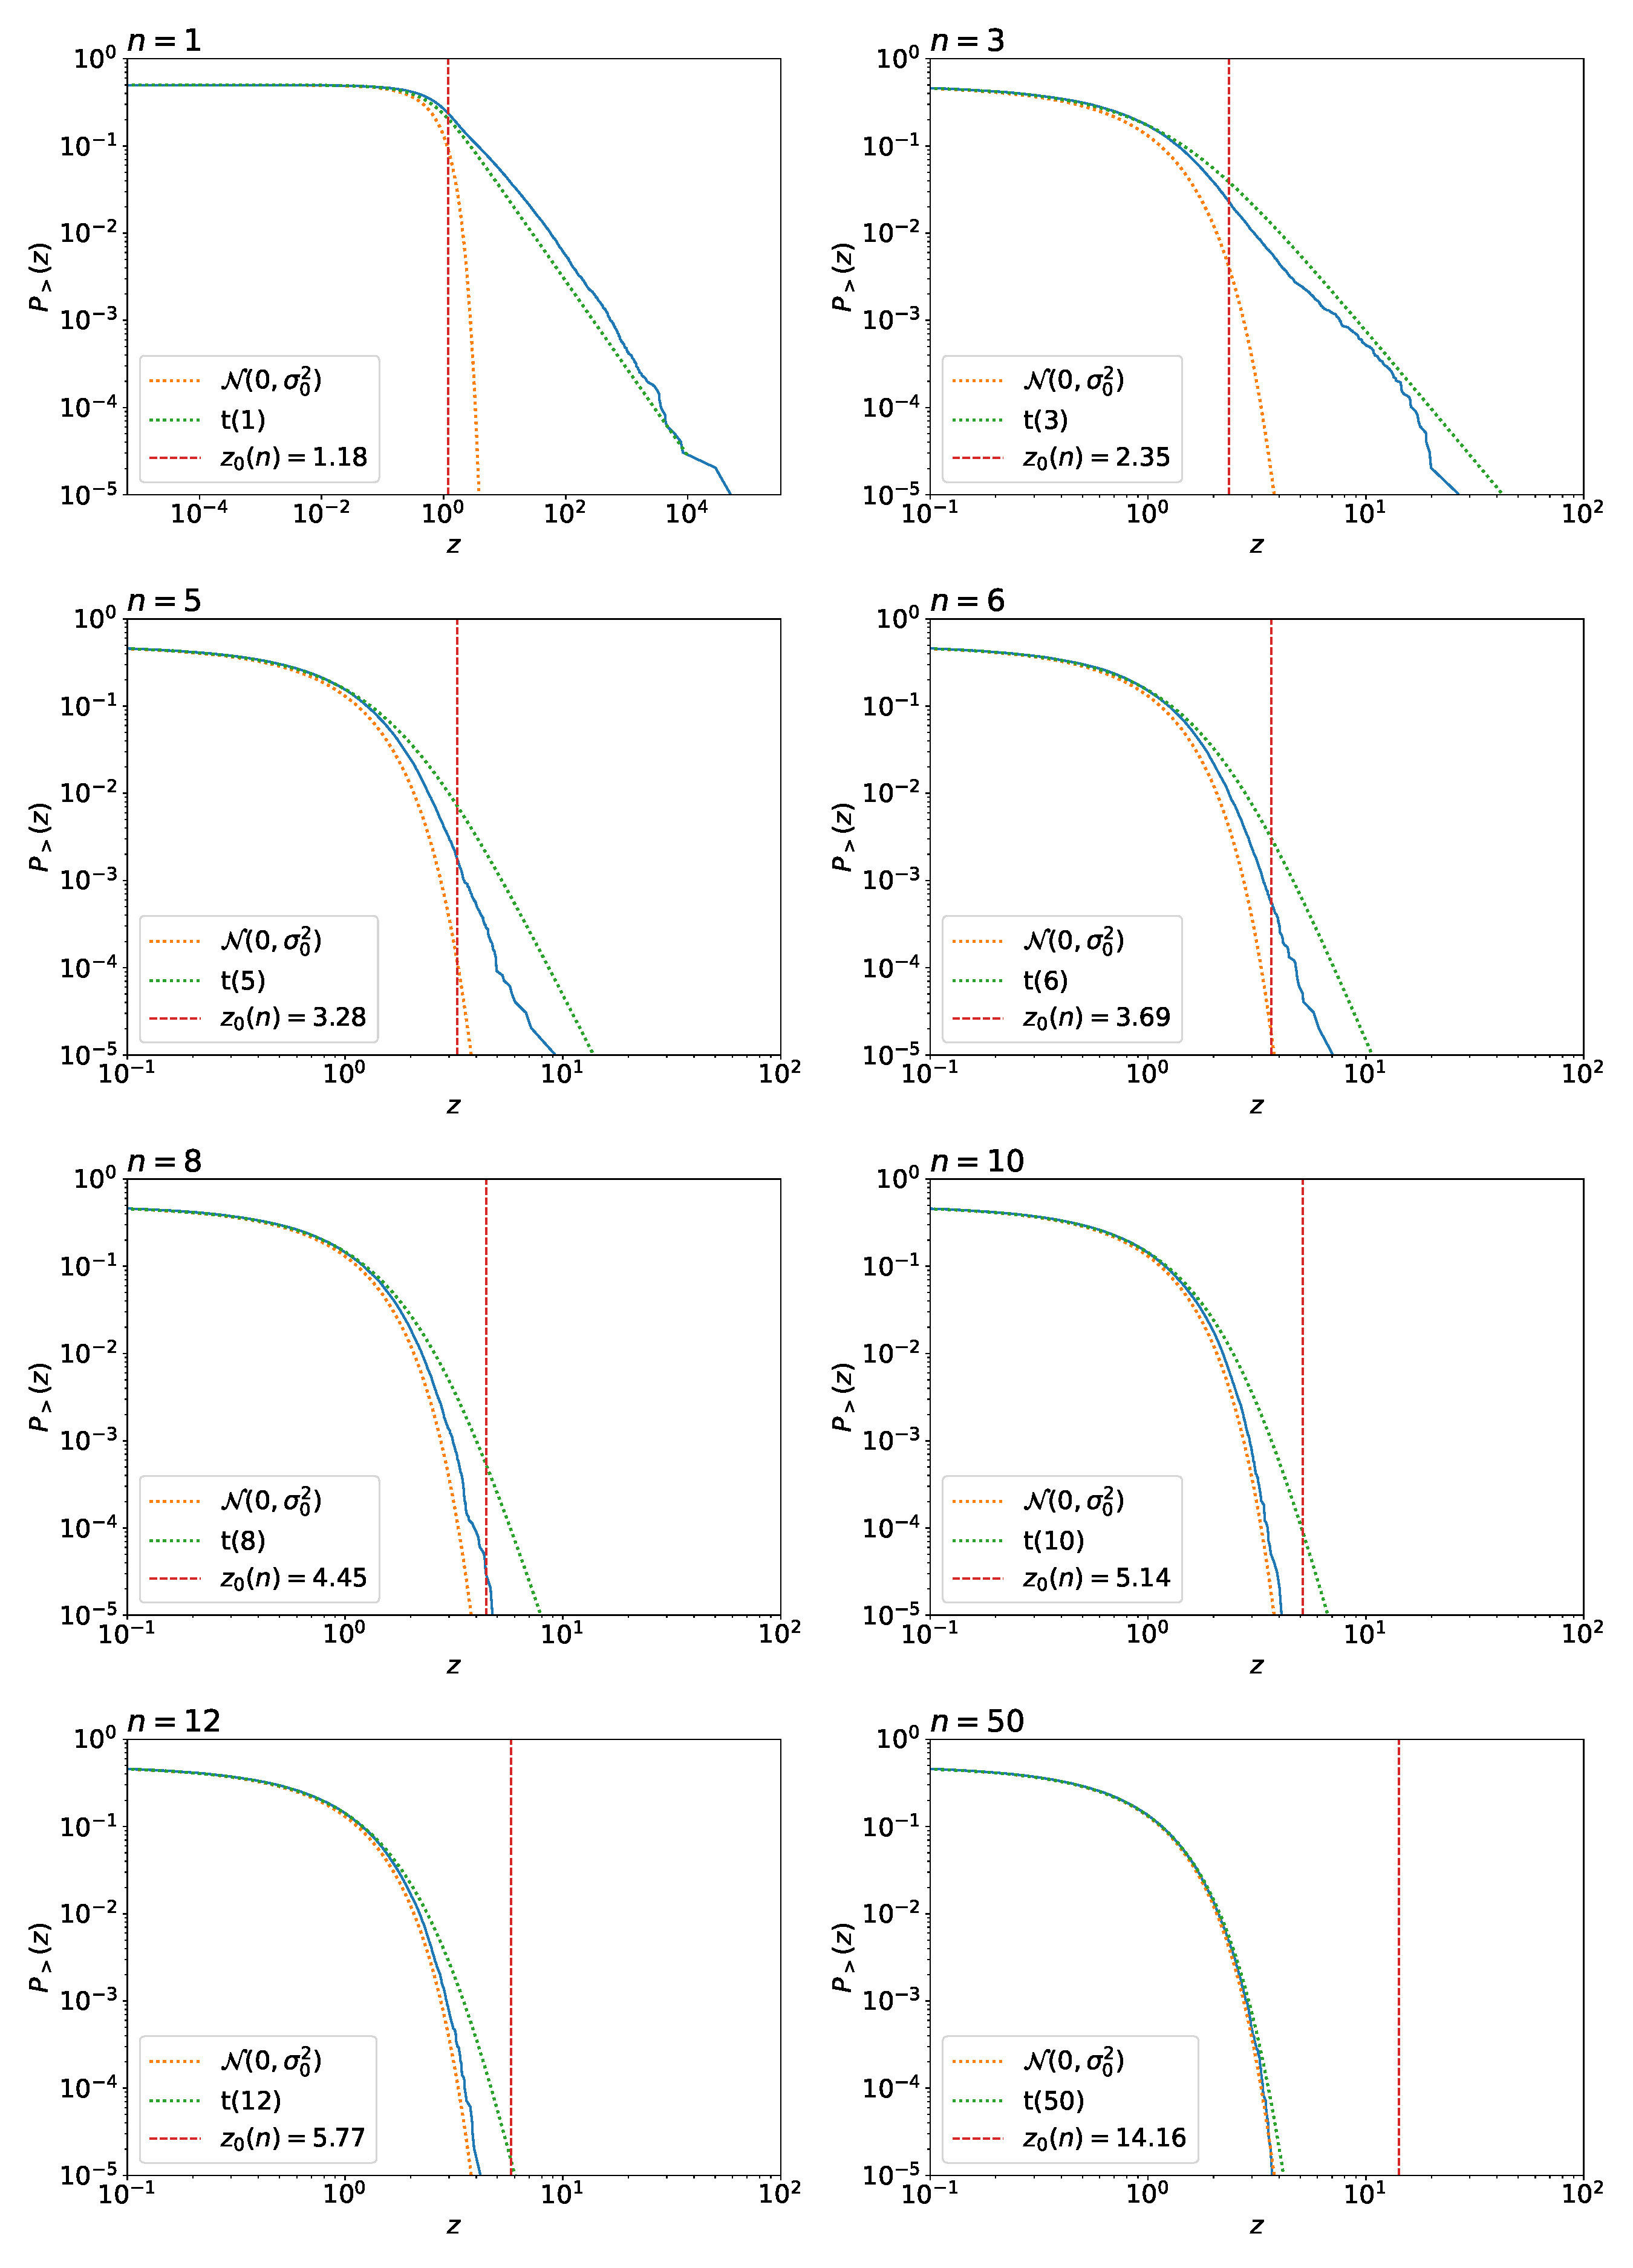
\includegraphics[width=1.2\textwidth]{Graphs/CCDF_n.pdf}}
	\caption{Tail distribution of time series simulated with \eqref{eq:map} and \eqref{eq:controller_mle_n}. In orange and green, CCDF of $\N(0,\sigma_0^2)$ and $t(n)$ for reference. Red dashed line indicates the region of convergence toward a Gaussian $z_0(n)$. After this threshold the power tail remains \eqref{eq:z0}.}
	\label{fig:ccdf_n}
\end{figure}


\bibliography{ref.bib}
%-----------------------------------------------------------
\end{document}